\documentclass[conference,a4paper]{IEEEtran}
\IEEEoverridecommandlockouts
\usepackage{cite}
\usepackage{amsmath,amssymb,amsfonts}
\usepackage{graphicx}
\usepackage{textcomp}
\usepackage{xcolor}
\usepackage{booktabs}
\usepackage{xurl}
\usepackage{pgfplots}
\pgfplotsset{compat=1.18}

\begin{document}

\title{Zero-Days in Your Pocket: Comparing Android and iOS Under Real-World Exploitation}

\author{\IEEEauthorblockN{Author Name}
\IEEEauthorblockA{\textit{Faculty of Computer Science and Mathematics} \\
University of Passau\\
Passau, Germany \\
name@uni-passau.de}
}

\maketitle

\begin{abstract}
A zero-day vulnerability is exploited before any patch exists. On mobile
devices, where the phone holds payment credentials, private messages, and
location history, this class of flaw carries the highest risk. Android and
iOS dominate the market, but they are built and shipped differently: Android
is open source and reaches users through many manufacturers and update
channels, while iOS runs on closed hardware controlled by a single vendor.
This paper compares how the two platforms are affected by zero-days and how
they respond to them. We compiled data from Google's in-the-wild tracker,
vendor security bulletins, and the published literature, and compared Android
and iOS along five dimensions: disclosure and patch delivery, ecosystem
fragmentation, exploit mitigations, hardware-backed defenses, and documented
in-the-wild exploitation. The synthesis finds that iOS accounts for most
documented mobile zero-day exploitation, that Android's fragmented update
chain slows patch delivery, and that both platforms now anchor their defenses
in dedicated hardware. We close with implications for users, vendors, and
future research.
\end{abstract}

\begin{IEEEkeywords}
Android, iOS, hardware security, mobile security, vulnerability management, zero-day exploit
\end{IEEEkeywords}

\section{Introduction}
In January 2026, Google's Project Zero published a working zero-click exploit
chain for a Pixel 9 phone~\cite{silvanovich2026pixel}. An incoming audio
message to Google Messages was decoded by a vulnerable Dolby decoder
(CVE-2025-54957) before the user touched the device. The authors built the
chain to study defensive options, and it shows what a well-funded attacker
can do to a fully patched, current-generation device. Criminal capability on
iOS is equally concrete: in 2025, the Citizen Lab forensically confirmed that
Graphite, the spyware product of Paragon Solutions, had infected the iPhones
of European journalists through a zero-click iMessage exploit
(CVE-2025-43200)~\cite{marczak2025graphite}. Neither case is unusual in kind.
Google's Threat Intelligence Group (GTIG) tracked 97 zero-day vulnerabilities
exploited in the wild in 2023, 75 in 2024, and 90 again in
2025~\cite{gtig2023review, charrier2025zeroday, gtig2026review}, and it observed that
attackers chained several zero-days together almost exclusively against
mobile devices~\cite{charrier2025zeroday}. The exposure is broad: Android
runs on roughly 69\% of smartphones worldwide~\cite{statcounter2026}, and
Apple reported more than 2.5 billion active devices in January
2026~\cite{apple2026devices}.

A zero-day is a flaw that is exploited before a patch exists, so no signature
or prior update can stop the first attack~\cite{nist2022zeroday}. How much
damage that first attack does, and how fast it stops working, is decided by
engineering choices made years earlier. Android is developed as open source,
extended by device makers, and delivered to users through
manufacturer-specific update channels. Google publishes a monthly security
bulletin, but applying it is optional for each
manufacturer~\cite{aospbulletin2026}. iOS ships on hardware that Apple
controls end to end, with one update pipeline and security fixes pushed
directly to users, most recently as rapid security
responses~\cite{applesecurity2026, applersr2026}. These structural
differences should be visible in the zero-day record: in how often each
platform is exploited, how quickly fixes reach devices, and how far an
attacker gets before hardware defenses stop them.

Both vendors have moved the anchors of that defense into dedicated hardware.
Android pairs ARM TrustZone-based trusted execution environments with
verified boot and hardware-backed keystores~\cite{aospverifiedboot2026,
aospkeystore2026}. Apple roots its boot chain in its own silicon and isolates
secrets in the Secure Enclave~\cite{applesecurity2026}. A modern mobile
exploit chain must therefore do more than corrupt memory: it has to bypass
mechanisms built for exactly this purpose. A comparison of zero-day exposure
that ignores this layer misses half the story.

Published work covers parts of this space. Surveys exist for Android malware
and its defenses, for iOS exploitation techniques, and industry reports track
zero-day counts year by year. What is missing is a structured, current
comparison across both platforms that includes the hardware layer. This
paper contributes a comparison framework with five dimensions for the
zero-day posture of mobile operating systems; a synthesis of in-the-wild
exploitation and patching data from 2019 through 2026, drawn from public
trackers and vendor bulletins; and an evaluation that places hardware-backed
defenses inside that comparison and derives implications for vendors and
researchers.

The rest of the paper is organized as follows. Section~II provides background
on zero-day terminology and the security architectures of Android and iOS.
Section~III reviews related work. Section~IV describes the comparison
framework and the data collection. Section~V evaluates the two platforms and
discusses threats to validity. Section~VI concludes.

\section{Background}

\subsection{Zero-Day Fundamentals}
A zero-day vulnerability is a flaw exploited before the vendor knows about
it, so no patch exists during the first attacks~\cite{nist2022zeroday}. Its
life cycle runs from private discovery through active exploitation to public
disclosure, patch release, and eventual loss of value as the installed base
updates; Fig.~\ref{fig:lifecycle} sketches the timeline. Two properties
make this cycle dangerous. First, exploitation is
invisible for a long time: Bilge and Dumitras measured 18 vulnerabilities
that were exploited in the wild for an average of 312 days before
disclosure, with the longest case at about two and a half
years~\cite{bilge2012before}. Second, disclosure changes the threat rather
than ending it; the same study found attack volume rose by up to five
orders of magnitude after details became public~\cite{bilge2012before}.

\begin{figure}[htbp]
\centering
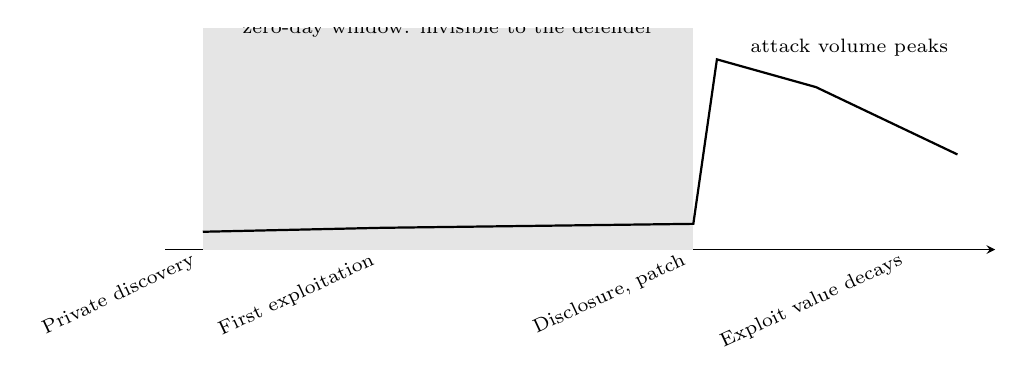
\begin{tikzpicture}
\begin{axis}[
    width=\columnwidth,
    height=4.4cm,
    xmin=0, xmax=8.8,
    ymin=0, ymax=5.6,
    axis x line=bottom,
    axis y line=none,
    xtick={0.4,2.3,5.6,7.9},
    xticklabels={{Private discovery},{First exploitation},{Disclosure{,} patch},{Exploit value decays}},
    xticklabel style={rotate=25, anchor=east, font=\scriptsize, align=left},
    tick style={draw=none},
]
\path[fill=gray!20] (axis cs:0.4,0) rectangle (axis cs:5.6,5.6);
\addplot[thick] coordinates {(0.4,0.45) (2.3,0.55) (5.6,0.65) (5.85,4.8) (6.9,4.1) (8.4,2.4)};
\node[font=\scriptsize, anchor=south] at (axis cs:3.0,5.1) {zero-day window: invisible to the defender};
\node[font=\scriptsize, anchor=west] at (axis cs:6.1,5.1) {attack volume peaks};
\end{axis}
\end{tikzpicture}
\caption{Life cycle of a zero-day vulnerability. Attack volume is
schematic, following the measurements of Bilge and
Dumitras~\cite{bilge2012before}: low and invisible during the shaded
zero-day window, which averaged 312 days, peaking by up to five orders of
magnitude after disclosure, then decaying as the installed base patches.}
\label{fig:lifecycle}
\end{figure} The
RAND Corporation's study of more than 200 zero-days additionally found no
evidence that zero-day exploits age quickly; many remained useful long
after vendors patched them, because deployment of patches
lagged~\cite{ablon2017zero}. Disclosure practice reflects this urgency:
Project Zero gives vendors 90 days and cuts the deadline to seven days
when a bug is found being exploited against real users~\cite{p0policy}.
Detection is the bottleneck of the whole field: Project Zero's tracker
records, on average, a newly discovered in-the-wild exploit every 17
days~\cite{p0tracker}, and each discovery means attackers were there
first. Mobile platforms are a special case on both ends. Attacks are
delivered without any user interaction, and Google's Threat Intelligence
Group (GTIG) found that exploit chains combining several zero-days were
aimed at mobile devices in about 90\% of observed
cases~\cite{charrier2025zeroday}.

\subsection{Android Security Architecture}
Android is an open-source platform that Google does not ship to users
directly. Device manufacturers adapt the Android Open Source Project (AOSP)
to their hardware, and carriers sit between them and the subscriber. Google
has published a monthly security bulletin since 2015 and requires a
security patch level (SPL) with each release, but integrating the fixes
into shipping devices is the manufacturers' work~\cite{aospbulletin2026}.
The measurable cost of this structure is delay. Jones et al.\ studied the
deployment of Android security updates across manufacturers, carriers, and
users, and found a median latency of 24 days before an update even begins
to roll out, followed by further device-side delays~\cite{jones2020deploying}.
Zhang et al.\ traced kernel security patches through the same ecosystem and
documented the same pattern: OEM schedules introduce avoidable
delay~\cite{zhang2021kernel}. Google has narrowed the gap architecturally.
Project Treble (Android 8.0, 2017) separated the OS framework from
silicon-specific code, and modular system components, delivered as Google
Play system updates since Android 10 (2019), let Google patch parts of the
OS directly on every device~\cite{mainline2019}. Support contracts vary by
manufacturer; Google's own Pixel 8 series carries a seven-year
commitment~\cite{pixel2023support}. The hardware layer holds the deepest
anchors: verified boot checks each stage of startup against a hardware root
of trust~\cite{aospverifiedboot2026}, ARM TrustZone isolates trusted
execution environments (TEEs) from the main OS~\cite{pinto2019demystifying},
and keys can reside in a separate secure processor via the hardware-backed
keystore, such as the Titan M chip introduced with the Pixel
3~\cite{aospkeystore2026, titanm2018}.

\subsection{iOS Security Architecture}
iOS takes the opposite shape: Apple writes the OS, builds the SoC, reviews
every App Store submission, and pushes updates to all supported devices
through one channel~\cite{applesecurity2026}. The same guide documents the
mitigation stack that has accumulated against zero-day exploitation.
BlastDoor, added in iOS 14, parses untrusted Messages content inside a
tightly sandboxed service that Project Zero's analysis credited with
shrinking the iMessage attack surface~\cite{silvanovich2021imessage,
applesecurity2026}. Lockdown Mode (iOS 16, 2022) is an opt-in mode for
users facing mercenary spyware that disables the most exploitable
surfaces~\cite{lockdown2022}. Rapid Security Responses (iOS 16.4, 2023)
deliver security fixes between full OS releases~\cite{applersr2026}. The
hardware roots run deepest here: the immutable boot ROM anchors the boot
chain, the Secure Enclave isolates biometric data and cryptographic keys on
a dedicated coprocessor, ARM pointer authentication (A12, 2018) hardens
code against memory-corruption reuse, and the Page Protection Layer
(iOS 16) restricts modifications to kernel memory, with successors (SPTM,
TXM) extending this from iOS 17~\cite{applesecurity2026}. Every iPhone
ships with this stack; nothing depends on a third party integrating it.

\section{Related Work}

Research relevant to this paper falls into three groups.

\subsection{Empirical Zero-Day Studies}
Bilge and Dumitras pioneered the measurement of zero-day attacks in the
wild and quantified how long exploitation precedes
discovery~\cite{bilge2012before}. Ablon and Bogart described the economic
side: who buys zero-days, what they pay, and how long exploits stay
useful~\cite{ablon2017zero}. Since 2019, Google has published the
definitive exploitation corpus. Project Zero tracks every publicly known
in-the-wild zero-day in a public list~\cite{p0tracker}, and GTIG's annual
reviews break the counts down by vendor, product type, and
attacker~\cite{gtig2023review, charrier2025zeroday, gtig2026review}. These
sources describe what happened but stop short of comparing platforms
systematically.

\subsection{Platform Security Comparisons}
Faruki et al.\ surveyed Android's security mechanisms and malware
landscape~\cite{faruki2015android}. The closest work to ours is the
comparison by Garg and Baliyan, who contrasted Android and iOS across
architecture, app stores, permission models, and updates, and concluded
that Android's fragmented update ecosystem makes it the more vulnerable
platform~\cite{garg2021comparative}. Their study covers the state of both
systems through 2020. Several of the mechanisms this paper evaluates
(Lockdown Mode, Page Protection Layer, mature Google Play system updates)
postdate their analysis, and their data set contains no in-the-wild
exploitation counts.

\subsection{Hardware-Backed Security and Spyware Cases}
Pinto and Santos surveyed TrustZone-based TEEs~\cite{pinto2019demystifying},
and Cerdeira et al.\ systematized the vulnerabilities found in deployed
TEEs~\cite{cerdeira2020sok}. Forensic reports from the Citizen Lab document
individual iOS zero-day campaigns in technical depth, among them
FORCEDENTRY~\cite{marczak2021forcedentry} and the Paragon
campaigns~\cite{marczak2025graphite}, and Amnesty International's
methodology report established the indicators used to detect Pegasus
infections at scale~\cite{amnesty2021forensic}. Google Project Zero's own writing
covers both sides: the discovery of BlastDoor~\cite{silvanovich2021imessage}
and a full zero-click Android research chain~\cite{silvanovich2026pixel}.

The present work differs from all of the above in three ways. It compares
the two platforms on zero-days specifically rather than on security in
general; it draws on exploitation data from 2023 through 2026, after the
latest hardening rounds on both sides; and it places hardware-backed
defenses inside the comparison rather than treating them as a separate
literature.

\section{Implementation: Comparative Framework}

\subsection{Method}
The study is a literature meta-analysis. We collected sources in four
categories: annual in-the-wild exploitation reviews from
GTIG~\cite{gtig2023review, charrier2025zeroday, gtig2026review} and the
Project Zero tracker~\cite{p0tracker}; forensic case reports on mobile
spyware campaigns~\cite{marczak2021forcedentry, amnesty2021forensic,
marczak2025graphite};
official vendor documentation for security bulletins, platform security,
and update mechanisms~\cite{aospbulletin2026, applesecurity2026}; and
peer-reviewed empirical studies of mobile security and
patching~\cite{bilge2012before, jones2020deploying, zhang2021kernel,
garg2021comparative}. The window of interest is 2019 through 2026,
starting when continuous in-the-wild tracking became available. A source
was included if it documents a confirmed in-the-wild mobile zero-day, a
measured property of the disclosure or patching pipeline, or a deployed
defense mechanism on either platform. From each included source we
extracted, where applicable: the CVE identifier, platform, delivery
vector, fix version and date, measured patch latency, and the hardware or
software mechanism the case involved. The extraction produced the data
behind Section~V. The final corpus comprises three annual exploitation
reviews, the continuous Project Zero tracker, three forensic case reports,
seven peer-reviewed studies, and primary vendor documentation and
statistics, and the per-case extraction is archived in machine-readable
form alongside the collected sources.

A meta-analysis is the appropriate instrument here because the phenomenon
cannot be measured directly: re-running attacks against stock devices
would reproduce only the research side of the picture, while the criminal
side exists solely in detections and forensic reports. The method trades
experimental control for breadth, and its weaknesses are treated
explicitly in Section~\ref{sec:threats}.

\subsection{Framework}
The comparison framework has five dimensions, each tied to an observable
indicator. Table~\ref{tab:framework} defines them and lists what is
compared on each platform.

\begin{table}[htbp]
\caption{Comparison Framework: Dimensions and Indicators}
\begin{center}
\begin{tabular}{@{}p{1.55cm}p{2.9cm}p{2.9cm}@{}}
\toprule
\textbf{Dimension} & \textbf{Android indicator} & \textbf{iOS indicator} \\
\midrule
Disclosure and patch delivery & Monthly bulletin, SPL schedule, Play system updates & Direct OTA to all devices, Rapid Security Responses \\
Ecosystem fragmentation & OEM and carrier latency (days) & Single vendor, one channel \\
Exploit mitigations & SELinux, seccomp, app sandbox & BlastDoor, Lockdown Mode, PAC \\
Hardware-backed defenses & Verified boot, TrustZone TEE, Titan M keystore & Boot ROM, Secure Enclave, PPL \\
In-the-wild exploitation & ITW zero-day counts, CSV share & ITW zero-day counts, CSV share \\
\bottomrule
\end{tabular}
\label{tab:framework}
\end{center}
\end{table}

Dimensions one to three capture how fast a fix becomes protection and how
hard exploitation is once it starts. Dimension four captures the seminar's
theme: the anchors that survive even a fully compromised OS kernel.
Dimension five is the outcome measure, taken from the GTIG corpus, that
shows how the structural differences above translate into recorded
attacks. Applying an outcome measure alongside structural measures is what
distinguishes this framework from a feature checklist.

\textbf{Threat model.} We consider four actor classes, taken from the
attribution in the sources: state-sponsored espionage groups, which GTIG
consistently ranks among the most prolific zero-day
users~\cite{gtig2023review}; commercial surveillance vendors (CSVs),
which sell exploit chains to state customers~\cite{marczak2021forcedentry,
marczak2025graphite}; physical-access forensic toolmakers such as
Cellebrite~\cite{charrier2025zeroday}; and financially motivated
criminals, largely absent from the mobile record because their zero-day
targets lie in enterprise software~\cite{gtig2026review}. The attacker
starts remotely with no user interaction or, in the forensic class, with
the device in hand. Success means arbitrary code execution, and full
compromise requires defeating the hardware-backed boundary. The framework
scores defenses against exactly this progression.

\section{Evaluation}

\subsection{In-the-Wild Exploitation}
Table~\ref{tab:itw} summarizes the GTIG counts, and Fig.~\ref{fig:itw}
shows how small the mobile share of total exploitation is. Mobile
zero-days fell from 17 in 2023 to 9 in 2024 and rose again to 15 in
2025~\cite{gtig2023review, charrier2025zeroday, gtig2026review}. The
counts understate mobile's role: in 2024, exploit chains that combined
several zero-days targeted mobile devices in roughly 90\% of observed
cases~\cite{charrier2025zeroday}.

\begin{table}[htbp]
\caption{Zero-Days Exploited in the Wild, as First Reported by GTIG}
\begin{center}
\begin{tabular}{@{}lcccc@{}}
\toprule
\textbf{Year} & \textbf{Total ITW} & \textbf{Mobile} & \textbf{Android} & \textbf{Apple} \\
\midrule
2023 & 97 & 17 & 7 & $-$ \\
2024 & 75 & 9 & 7 & 5 \\
2025 & 90 & 15 & $-$ & $-$ \\
\bottomrule
\end{tabular}
\label{tab:itw}
\end{center}
\vspace{-2mm}
\footnotesize Dashes: per-vendor counts not itemized in that year's review. Later reviews revise past totals upward (2023 to 100, 2024 to 78) as exploitation is back-attributed~\cite{gtig2026review}, so every figure is a lower bound.
\end{table}

\begin{figure}[htbp]
\centering
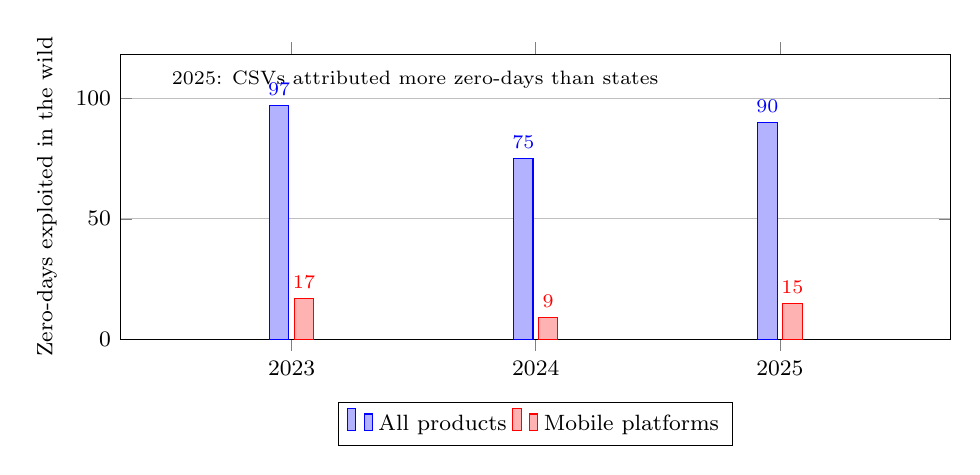
\begin{tikzpicture}
\begin{axis}[
    ybar,
    bar width=7pt,
    width=\columnwidth,
    height=5.2cm,
    ymin=0,
    symbolic x coords={2023,2024,2025},
    xtick=data,
    ylabel={Zero-days exploited in the wild},
    legend style={at={(0.5,-0.22)}, anchor=north, legend columns=2, font=\footnotesize},
    ymajorgrids=true,
    tick label style={font=\footnotesize},
    label style={font=\footnotesize},
    nodes near coords,
    every node near coord/.append style={font=\scriptsize},
    enlarge x limits=0.35,
    enlarge y limits={upper,value=0.22},
]
\addplot coordinates {(2023,97) (2024,75) (2025,90)};
\addplot coordinates {(2023,17) (2024,9) (2025,15)};
\legend{All products, Mobile platforms}
\node[font=\scriptsize, anchor=west] at (rel axis cs:0.05,0.91) {2025: CSVs attributed more zero-days than states};
\end{axis}
\end{tikzpicture}
\caption{In-the-wild zero-day counts per year. Mobile is a minority of
exploitation but carries almost all multi-zero-day chains.}
\label{fig:itw}
\end{figure}

Who exploits, and what, differs by platform. Commercial surveillance
vendors (CSVs) dominate this space: they were behind 75\% (13 of 17) of
the zero-days that hit Google products and Android ecosystem devices in
2023, and more than 60\% of the 37 browser and mobile zero-days that
year~\cite{gtig2023review}. In 2025, GTIG attributed more zero-days to
CSVs than to state-sponsored espionage groups for the first
time~\cite{gtig2026review}. The 2025 mobile rebound has identifiable
causes: researchers uncovered more complete chains, chains grew to three
or more vulnerabilities, and vendors such as Intellexa developed new
techniques to cross the security boundaries Apple had
added~\cite{gtig2026review}. Browsers show what successful platform
hardening looks like: they drew under 10\% of 2025 zero-days, a historic
low that GTIG credits to years of sandboxing and memory-safety
work~\cite{gtig2026review}. Mobile OS hardening has not produced a
comparable drop, and the case evidence below suggests why. On Android,
the exploited bugs concentrate in
third-party components, which scale one exploit across many device
makers: five of seven Android zero-days in 2023 and three of seven in
2024~\cite{charrier2025zeroday}.

Table~\ref{tab:cases} lists the four anchor cases, and
Fig.~\ref{fig:timeline} places their verified dates on one axis. The iOS
campaigns share a recipe, zero-click delivery followed by an emergency
fix, and FORCEDENTRY bypassed BlastDoor, the very sandbox added to stop
it~\cite{marczak2021forcedentry}. The Android cases bookend the spectrum:
a zero-click research chain through a third-party
decoder~\cite{silvanovich2026pixel} and a forensic tool needing physical
access~\cite{charrier2025zeroday}.

\begin{table}[htbp]
\caption{Documented In-the-Wild and Research Cases}
\begin{center}
\begin{tabular}{@{}p{2.1cm}p{1.1cm}p{2.3cm}p{1.25cm}@{}}
\toprule
\textbf{Case (actor)} & \textbf{Platform} & \textbf{Vector} & \textbf{Fix} \\
\midrule
FORCEDENTRY (NSO, 2021) & iOS & Zero-click iMessage, CVE-2021-30860 & iOS 14.8 \\
Graphite (Paragon, 2025) & iOS & Zero-click iMessage, CVE-2025-43200 & iOS 18.3.1 \\
Cellebrite chain (2024) & Android & Physical USB access, CVE-2024-53104 & Bul.\ Feb.\ 2025 \\
Pixel 9 chain (P0, 2026) & Android & Zero-click transcription, CVE-2025-54957 & Before disclosure \\
\bottomrule
\end{tabular}
\label{tab:cases}
\end{center}
\end{table}

\begin{figure}[htbp]
\centering
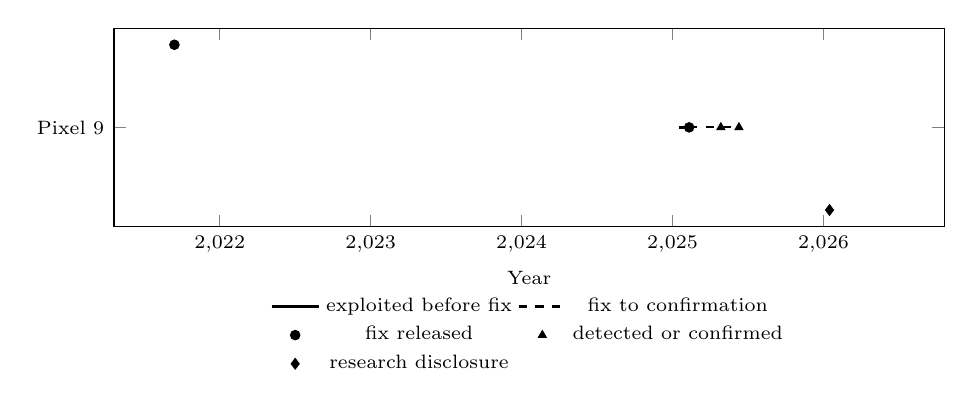
\begin{tikzpicture}
\begin{axis}[
    width=\columnwidth,
    height=4.1cm,
    symbolic y coords={P9,GPH,FE},
    ytick=data,
    yticklabels={{Pixel 9},{Graphite},{FORCEDENTRY}},
    yticklabel style={font=\scriptsize, align=left},
    xmin=2021.3, xmax=2026.8,
    xtick={2022,2023,2024,2025,2026},
    xticklabel style={font=\scriptsize},
    xlabel={Year}, xlabel style={font=\scriptsize},
    legend style={at={(0.5,-0.30)}, anchor=north, legend columns=2, font=\scriptsize, draw=none, fill=none},
]
\addplot[very thick] coordinates {(2025.04,GPH) (2025.11,GPH)};
\addlegendentry{exploited before fix}
\addplot[thick, dashed] coordinates {(2025.11,GPH) (2025.44,GPH)};
\addlegendentry{fix to confirmation}
\addplot[only marks, mark=*, mark size=1.7pt] coordinates {(2021.70,FE) (2025.11,GPH)};
\addlegendentry{fix released}
\addplot[only marks, mark=triangle*, mark size=1.6pt] coordinates {(2025.32,GPH) (2025.44,GPH)};
\addlegendentry{detected or confirmed}
\addplot[only marks, mark=diamond*, mark size=1.9pt] coordinates {(2026.04,P9)};
\addlegendentry{research disclosure}
\end{axis}
\end{tikzpicture}
\caption{Case timeline assembled from Table~\ref{tab:cases}. FORCEDENTRY
was captured and fixed on the same day, so its pre-detection span is
unknown. Graphite infections ran about a month before the iOS 18.3.1 fix,
and forensic confirmation followed four months later.}
\label{fig:timeline}
\end{figure}

\subsection{Applying the Framework}
Table~\ref{tab:applied} fills the five dimensions of Table~\ref{tab:framework}
with the evidence collected above.

\begin{table*}[htbp]
\caption{Framework Applied: Android and iOS Compared on the Five Dimensions}
\begin{center}
\begin{tabular}{@{}p{2.1cm}p{6.6cm}p{6.6cm}@{}}
\toprule
\textbf{Dimension} & \textbf{Android} & \textbf{iOS} \\
\midrule
Patch delivery & Monthly bulletin; OEMs integrate fixes; median 24-day rollout latency before updates even begin~\cite{jones2020deploying}; Play system updates patch some components directly~\cite{mainline2019} & One vendor, one channel; Rapid Security Responses push fixes between releases~\cite{applersr2026} \\
\addlinespace
Fragmentation & Hundreds of manufacturer and carrier variants; kernel patches propagate unevenly~\cite{zhang2021kernel}; Pixel 8 sets a 7-year ceiling~\cite{pixel2023support} & Single hardware and OS vendor; support horizon uniform across devices~\cite{applesecurity2026} \\
\addlinespace
Exploit mitigations & SELinux, seccomp, app sandbox; no platform-wide messaging sandbox; the Pixel 9 chain entered through a third-party decoder~\cite{silvanovich2026pixel} & BlastDoor isolates message parsing~\cite{silvanovich2021imessage}; Lockdown Mode for high-risk users~\cite{lockdown2022}; FORCEDENTRY shows bypasses are possible~\cite{marczak2021forcedentry} \\
\addlinespace
Hardware defenses & Verified boot and TrustZone broadly present~\cite{aospverifiedboot2026, pinto2019demystifying}; secure processors (Titan M) ship on some devices~\cite{titanm2018}; deployed TEEs have documented vulnerabilities~\cite{cerdeira2020sok} & Boot ROM, Secure Enclave, PAC, and PPL present on every device~\cite{applesecurity2026} \\
\addlinespace
In-the-wild outcome & 7 ITW zero-days in each of 2023 and 2024, mostly third-party components~\cite{charrier2025zeroday}; physical-access forensic chains~\cite{charrier2025zeroday} & Repeated zero-click CSV campaigns (2021, 2025)~\cite{marczak2021forcedentry, marczak2025graphite}; 5 ITW zero-days in 2024~\cite{charrier2025zeroday} \\
\bottomrule
\end{tabular}
\label{tab:applied}
\end{center}
\end{table*}

The synthesis runs against the older narrative that Android is simply the
less secure platform~\cite{garg2021comparative}. On delivery speed and
reach, iOS holds the advantage: a fix Apple ships reaches every supported
device, while the same Android fix waits on OEM integration, measured in
weeks before rollout even starts~\cite{jones2020deploying}. On attack
surface, the platforms fail differently. Android's exploited zero-days sit
mostly in third-party components, a structural consequence of the
ecosystem's openness; iOS draws sustained, sophisticated zero-click
campaigns from the spyware market, and its mitigation stack is exactly
what those campaigns must defeat. On hardware, both platforms anchor
their defenses in silicon, and the difference is universality: every
iPhone carries the boot ROM, Secure Enclave, and PPL, while Android's
deepest anchors (a discrete secure processor) depend on the device
maker. The Pixel 9 chain adds a third-party illustration of the same
point: the vulnerable Dolby decoder code also ships on Apple platforms,
where the same bug class was blunted in advance by the
\texttt{-fbounds-safety} compiler mitigation~\cite{silvanovich2026pixel}.
Garg and Baliyan's conclusion still holds for updates; it does not
hold for in-the-wild exploitation, where the more integrated platform is
the one spyware vendors keep paying for.

\subsection{Implications}
For users, the timing of updates matters in a specific way. The first
attack is largely unavoidable, because exploitation is invisible for
months, but the wave after disclosure is not: attack volume grew by up to
five orders of magnitude once details became public in the measurement of
Bilge and Dumitras~\cite{bilge2012before}, so updating promptly removes
most of the real-world risk. Users facing targeted spyware have one
further option on iOS that Android lacks platform-wide: Lockdown Mode
trades functionality for a smaller attack surface~\cite{lockdown2022}.
For vendors, the evidence points to two levers. Shortening the path from
fix to installed base is the first, where Apple's direct channel and
Android's modular system updates both matter~\cite{applersr2026,
mainline2019}. Governing third-party components is the second, since they
supplied most of the exploited Android bugs. For researchers and
regulators, the binding constraint is detection: every count in this
paper is an exploitation that someone happened to
notice~\cite{p0tracker}, and update-focused regulation can only work
through the patching levers already discussed.

\subsection{Threats to Validity}\label{sec:threats}
In-the-wild counts are detections, not attacks: an exploit used quietly
against few targets can stay invisible, and mobile forensics skew toward
high-value victims, which may inflate iOS's visibility relative to
Android. Attribution to actor classes (CSV, state-sponsored) carries
uncertainty in the underlying reports. GTIG revises past-year counts
upward as new evidence arrives, so all totals are lower bounds. A
sensitivity check under the latest attribution (100 for 2023, 78 for
2024) changes no conclusion: mobile remains a small minority of
exploitation, the per-vendor ordering stands, and the CSV milestone is a
2025 event under either base. Vendor
transparency differs; we compare the two platforms with the best public
reporting, which limits generalization to other mobile systems. Finally,
cross-platform messaging apps blur the boundary: the Paragon campaign
used a WhatsApp flaw alongside the iOS exploit~\cite{marczak2025graphite},
and such bugs are not cleanly attributable to either OS.

\section{Conclusion and Future Work}
This paper compared Android and iOS through a five-dimension framework
covering disclosure and patch delivery, fragmentation, exploit
mitigations, hardware-backed defenses, and documented in-the-wild
exploitation. Three findings stand out. First, the platforms fail
differently: Android's zero-day exposure is dominated by fragmented patch
delivery and third-party components, while iOS attracts repeated
zero-click chains from commercial surveillance vendors. Second, patch
speed differs structurally: iOS delivers fixes directly to every
supported device, whereas Android updates wait on manufacturer
integration with a measured median latency of 24 days. Third, both
platforms now anchor their defenses in dedicated hardware, differing
mainly in whether every device ships the full stack. The evidence base is
detection-limited, so the counts should be read as lower bounds. Future
work should track the effect of memory tagging on exploit costs as it
rolls out, examine regulation such as the EU Cyber Resilience Act as an
update-forcing mechanism for the Android ecosystem, and extend the
framework to additional mobile operating systems.

\bibliographystyle{IEEEtran}
\bibliography{references}

\end{document}
